\chapter{Descripci\'on de la implentaci\'on} % (fold)
\label{cha:descripcion_de_la_implentacion}



  % la aplicacion se realizo sobre ruby on rails
  La aplicacion a desarrollar requeria de implementar un sistema de geolocalizaion, para tal motivo primeramente se procedio a generar un mapa de rutas sobre la cual escoger las herramientas mas apropiadas para la realizacion de la aplicacion.

  \section{Generaci\'on de las rutas} % (fold)
  \label{sec:generacion_de_las_rutas}
    Se procedio a trazar un mapa de rutas del campus de la Universidad Mayor de San Simon, para tal efecto se necesito de un GPS, el unico requisito del GPS es la posibilidad de grabar en su memoria la ruta que se camina. El GPS usado fue un Garmin Nuvi 1300, es un GPS basico pero cumple con el requisito, los archivos generados son gpx, es basicamente un fichero XML estandar para compartir datos entre GPS's.
    Posteriormente
    el archivo gpx necesita ser editado por un Sistema de Informacion Geografica, se uso QGis que es un SIG open sorce con licensia  GNU GPL multiplataforma. QGIs me permitio editar la ruta generada por el GPS, que al no ser exacto, era necesario este paso, generando un archivo shapefile, el cual es el formato estandar para manejar datos geograficos espaciales.

    \begin{figure}[!ht]
      \begin{center}
        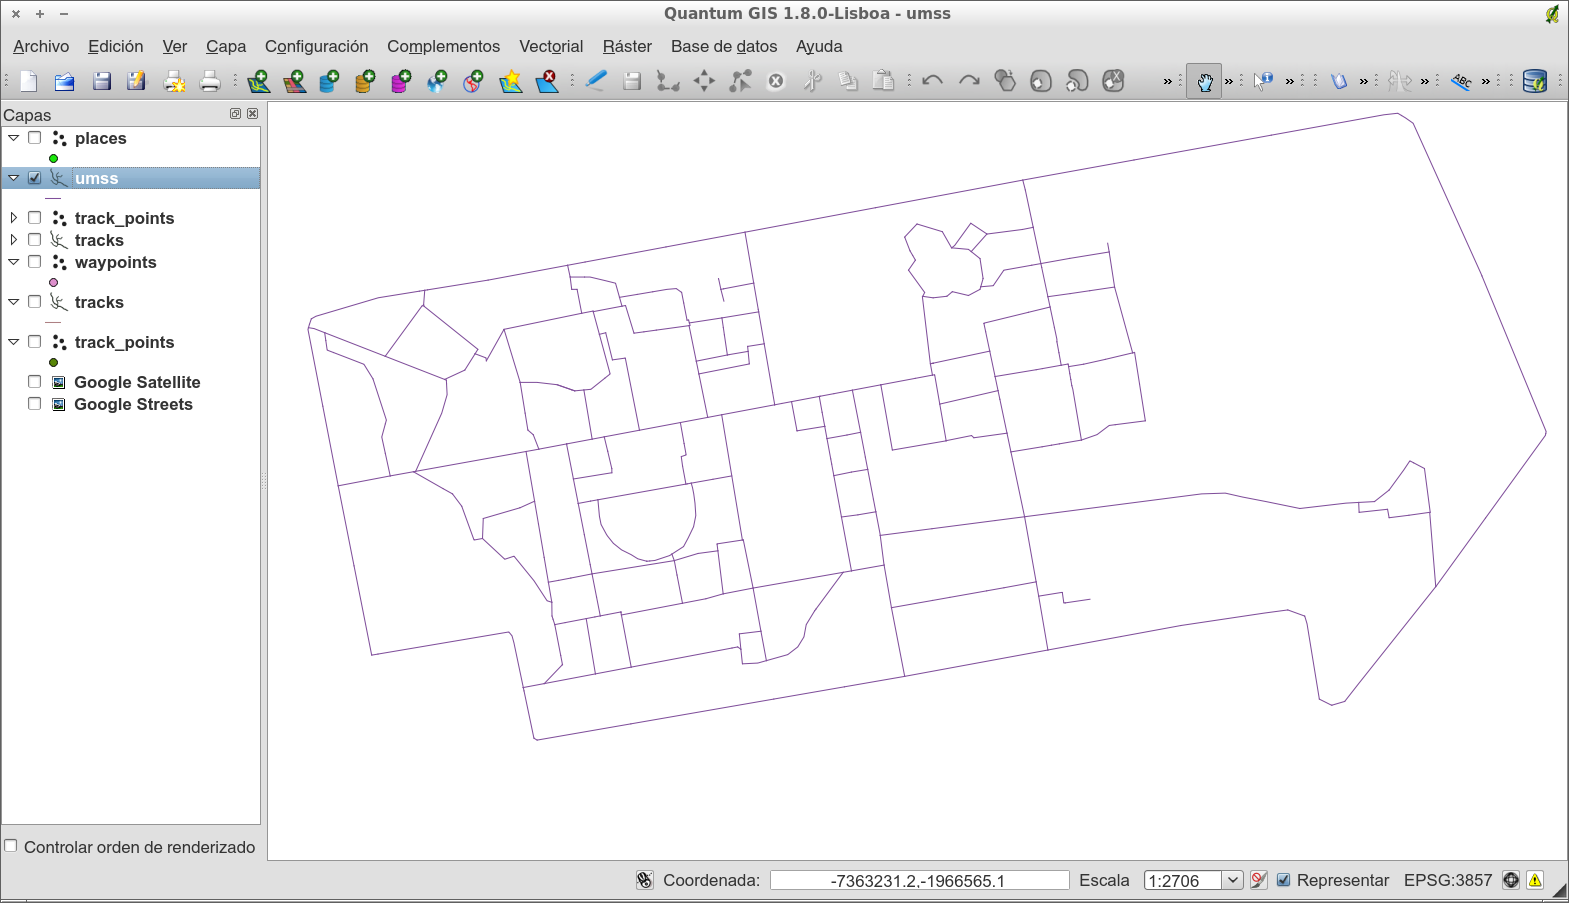
\includegraphics[width=0.8\textwidth]{rutas_qgis}
      \end{center}
      \caption{Rutas del Campus de la UMSS en QGis}
      \label{fig:rutas}
    \end{figure}

    El mapa generado con las rutas cumple con las caracteristicas de un grafo ponderado no-dirigido en el que el costo o peso de las aristas es la distacia entre los nodos y los nodos son los puntos de interseccion de las rutas. Por lo tanto se puede implentar el algoritmo de Dijkstra para encontrar el camino minimo.

  % section generacion_de_las_rutas (end)
  \section{Lectura de los archivos Shapefile} % (fold)
  \label{sec:lectura_de_los_archivos_shapefile}
    Es necesario cargar la base de datos PostGis con los shapefiles generados por QGis y para eso se uso la gema RGeo y con el siguiente metodo escrito en Ruby se carga los archivos shapefile en la base de datos.

    \begin{center}
      \begin{verbatim}
  def self.load_shapefile(path)
    RGeo::Shapefile::Reader.open(path, factory: FACTORY) do |file|
      file.each do |record|
        way = record.geometry.projection
        ruta = Way.create(name: record['id'],
                          dist: way.length,
                          the_geom: way[0])
      end
    end
  end
      \end{verbatim}
    \end{center}

  % section lectura_de_los_archivos_shapefile (end)
  \section{Los lugares} % (fold)
  \label{sec:los_lugares}
    Los lugares o sitios de interes se crean atraves de la aplicacion, ingresando a la seccion de \emph{Nuevo lugar}, en donde es necesario llenar el formulario y hacer un click sobre el mapa en el sitio que se desea registrat el nuevo lugar.

    \begin{figure}[!ht]
      \begin{center}
        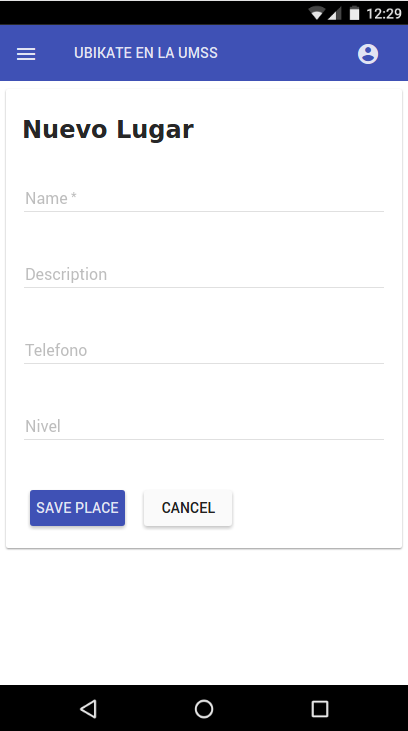
\includegraphics[width=0.8\textwidth]{new_place}
      \end{center}
      \caption{Registro de Nuevos lugares}
      \label{fig:new_place}
    \end{figure}
    % pero para fines practicos se registraron inicialmente unos 5x lugares mediante un shapefile
    \subsection{La geolocalizacion de los lugares} % (fold)
    \label{subsec:la_geolocalizacion_de_los_lugares}
      % Como creo dentro de rails un lugar.
      Para que Rails cree un lugar es necesario los siguentes pasos:
        \begin{itemize}
          \item Declarar un objeto que maneja la proyeci\'on \\
          \verb+ FACTORY = RGeo::Geographic.simple_mercator_factory +
          \item Declarar el atributo encargado de manejar el dato espacial, mediante el metodo \emph{set\_rgeo\_factory\_for\_column} especificando la proyeci\'on. \verb|set_rgeo_factory_for_column(:coord, FACTORY.projection_factory)|
          \item LLamar a al funcion \emph{create\_coord} cuando se crea un nuevo lugar, siempre teniendo en cuenta la proyecion en la cual se reciben los datos (\emph{lon} y \emph{lat} se reciben del lado del cliente en WS84) y proyectarlo para guardarlo correctamente en la base de datos (\emph{coord} esta en la proyecion EPSG 3785).
          % \begin{center}
          \begin{verbatim}
    def create_coord
      if self.new_record?
        self.coord = FACTORY.point(lon, lat).projection
      else
        p self.coord
      end
    end
          \end{verbatim}
          % \end{center}
        \end{itemize}


    % section la_geolocalizacion_de_los_lugares (end)

  % section los_lugares (end)
  \section{Modelo de base de datos} % (fold)
  \label{sec:modelo_de_base_de_datos}

  % section modelo_de_base_de_datos (end)
  \section{Camino minimo} % (fold)
  \label{sec:camino_minimo}

    Una ves se tienen las rutas en la base de datos es necesario realizar algunos pasos previos para encontrar el camino minimo, pgRouting requiere de una tabla en la especifica todos los vertices existentes. Toma como argumentos la tabla de la cual se debe extraer los vertices (ways), la distancia de tolerancia (0.001), el atributo espacial (the\_geom) y su id (gid)

    \begin{center}
      \begin{verbatim}
      SELECT assign_vertex_id('ways', 0.001, 'the_geom', 'gid');
      \end{verbatim}
    \end{center}

    Al tener ya lista la base de datos, se procede a llamar a la funcion \emph{shortest\_path} del modulo PgRouting  de PostGis, el cual implementa el algoritmo de Dijkstra para encontrar el camino minimo.

    En una computadora AMD K6 de 1.8 GHz, de 346 vertices se tiene el siguiente dato

    \begin{center}
      \begin{verbatim}
-- Executing query:
SELECT  * from  shortest_path('select gid as id,
                              source::integer,
                              target::integer,
                              dist::double precision as cost from ways',
                              20, 299 ,
                              false, false)
Total query runtime: 11 ms.
31 rows retrieved.
      \end{verbatim}
    \end{center}

    La funcion shortest\_path toma como variables el id del vertice origen (20), y el vertice destino (299).


  % section camino_minimo (end)

  \section{Modelos ?} % (fold)
  \label{sec:modelos_}

  % section modelos_ (end)
  \section{Diagrama de casos de uso ?} % (fold)
  \label{sec:diagrama_de_casos_de_uso_}

  % section diagrama_de_casos_de_uso_ (end)







% chapter descripcion_de_la_implentacion (end)


% la red social en la que los usuarios comparten las fotos de los sitios que visitan.
